\documentclass[11pt,a4paper]{report}

\usepackage[T1]{fontenc}


\setcounter{secnumdepth}{1}
\setcounter{tocdepth}{3}
\setlength{\parskip}{\smallskipamount}
\setlength{\parindent}{0pt}

% Customization file for the titlepage and document
%************************************************************
% Required stuff
%************************************************************
\usepackage[T1]{fontenc}
\usepackage[english]{babel}
\usepackage{graphicx}
\usepackage{euler}
\usepackage[detect-all]{siunitx}
\usepackage{sectsty}
\usepackage[font={footnotesize }]{caption}
\usepackage{multicol}
\usepackage{prettyref}
\usepackage[scale=0.75]{geometry}
\usepackage[utf8]{inputenc}
\usepackage[hyphens]{url}
\usepackage[unicode=true,bookmarks=true,bookmarksnumbered=false,bookmarksopen=false,breaklinks=false,pdfborder={0 0 1},backref=false,colorlinks=false]{hyperref}
\usepackage{datetime}
\usepackage{float}
\usepackage[nointegrals]{wasysym}
\usepackage{amsmath}
%Bibliography
\usepackage{etoolbox}
% Acronyms
\usepackage[acronym,nonumberlist,nopostdot,section=section,toc,numberedsection]{glossaries}

\allsectionsfont{\rmfamily}

% Page customization
\usepackage{fancyhdr}
\pagestyle{fancy}

% Color
\usepackage{color}
\definecolor{light-gray}{gray}{0.85}
\definecolor{dark-gray}{gray}{0.75}

\fancyhead{}  % clear all header fields
\fancyhead[LO,RE]{\rule[-2ex]{0pt}{2ex}\fontsize{9}{11} \selectfont \myPhase : \myTitle}
\fancyhead[CO,C]{\fontsize{9}{11} \selectfont \myIPT}
\fancyfoot{}  % clear all footer fields
\fancyfoot[RO,LE]{\fontsize{6}{11} \selectfont 
\includegraphics[height=0.2cm]{gfx/CC} This work is licensed under a Creative Commons Attribution-ShareAlike 4.0 International License.}
\fancyheadoffset[L,R]{0.2pt}
\renewcommand{\headrulewidth}{0.2pt}
\renewcommand{\footrulewidth}{0.2pt}
\renewcommand{\headrule}{\hbox to\headwidth{%
   \leaders\hrule height \headrulewidth\hfill}}
\renewcommand{\footrule}{\hbox to\headwidth{%
    \leaders\hrule height \headrulewidth\hfill}}
\hypersetup{colorlinks=true, linkcolor=blue ,linktoc=page,citecolor=black}

%************************************************************
% Redefining numbering for sections
%************************************************************
\renewcommand*\thesection{\arabic{section}}

%************************************************************
% Defining useful commands
%************************************************************
\newcommand{\norm}[1]{\left\lVert#1\right\rVert}

%************************************************************
% Cross reference set-up
%************************************************************
\newrefformat{tab}{Table\,\ref{#1}}
\newrefformat{fig}{Figure\,\ref{#1}}
\newrefformat{eq}{Eq.\,\textup{(\ref{#1})}}
\newrefformat{sec}{Sec.\,\ref{#1}}
\newrefformat{sub}{Sec.\,\ref{#1}}

%************************************************************
% Fancy stuff
%************************************************************
\newcommand{\titlecap}[1]{\Huge{\textrm{#1}}}
\newcommand{\subtitlecap}[1]{\Large{\textsc{#1}}}
\newcommand{\sscap}[1]{\textbf{#1}}
\newcommand{\strong}[1]{\textbf{#1}}
\setlength{\headheight}{60pt} %%or

%************************************************************
% Helpful stuff to modify here, not in the LyX Document
%************************************************************
\newcommand{\myDate}{\today}
\newcommand{\myGroup}{}
\newcommand{\myUrl}{\url{https://github.com/fcuzzocrea/SADC2017}}
\newcommand{\myUni}{}
\newcommand{\myPhase}{Spacecraft Attitude Dynamics and Control}
\newcommand{\myProject}{}
\newcommand{\myIPT}{}
\newcommand{\myTitle}{Assignment Report}
\newcommand{\myAuthor}{Francescodario Cuzzocrea}
\newcommand{\myEmail}{francescodario.cuzzocrea@mail.polimi.it}

\newcommand{\mail}[1]{\href{mailto:#1}{\texttt{#1}}}


\makeatother

\begin{document}

\thispagestyle{empty}
\pdfbookmark{Titlepage}{Titlepage}

\vspace{3cm}
\begin{center}
\bigskip
\Large{\myDate}
\vspace{0.5cm}

{\titlecap{\myProject} \\
\vspace{0.3cm}
\titlecap{\myPhase}}\\
\vspace{0.4cm}
\rule{\linewidth}{0.5mm}
\titlecap{\myTitle}


\vfill

\begin{tabular}{cc}
\hspace{2.5cm}
\parbox{0.3\textwidth}{
\includegraphics[height=7cm]{gfx/Polimi}}
&
\parbox{0.7\textwidth}{{\subtitlecap{\myIPT}} \\

					{\normalsize
						\textrm{\myGroup \\
						\myUni \\
						\textbf{Author}: {\myAuthor}\\
						\textbf{E-Mail}: {\myEmail}}}}\\
\end{tabular}
\end{center}
\clearpage

%*******************************************************
% Titleback
%*******************************************************
\thispagestyle{empty}

\hfill
\vspace{5cm}
\strong{ }\\
The following report will contain the procedure and the mathematical models used to simulate the behaviour a 6U Cubesat in a LEO orbit.
The sensor installed on the cubesat are a tri-axial magnetometer and a tri-axial gyroscope. 
The actuators installed on the cubesat to control the attitude are 3 magnetic torquers and a reaction wheel.

The latest version of the simulator can be found at : https://github.com/fcuzzocrea/SADC2017

\vfill

\begin{multicols}{2}
\medskip
\noindent{\sscap{Website}}: \\
\url{https://github.com/fcuzzocrea/SADC2017}

\end{multicols}
\vspace{1cm}
\hrule
\bigskip
\clearpage


\pagenumbering{roman}
\tableofcontents{}

\clearpage{}

\pagenumbering{arabic}
\setcounter{page}{3}

\chapter{Parameters and Mission Requirements}
In this chapter the parameters used to model and simulate the behavior of the assigned spacecraft will be defined starting from the customer requirements.\\
The parameters are divided in four main categories : 

\begin{itemize}
 \item Orbital Parameters
 \item Structural Parameters
 \item Sensors Parameters
 \item Actuators Parameters
 \item External Disturbances Parameters
\end{itemize}

\section{Customer Requirements}
The requirement placed from the customer for this mission are :

\begin{itemize}
 \item de-tumble Spacecraft after launcher injection\\
 \item perform Earth Pointing with \ang{0.1} accuracy\\
\end{itemize}

De-tumble a spacecraft means to reduce it's angular velocity to values which are comparable to the orbit's mean motion.\\
After the de-tumbling phase the spacecraft must be able to perform a slew maneuver in order to reorient itself to point the desired location on Earth's surface.\\

\section{Orbital Parameters}
The mission required by the customer is to perform Earth pointing. \\   
Only the altitude of the target orbit has be assigned by the customer. The other orbital parameters have been chosen as follows : 

\begin{table}[H]
	\centering
	\begin{tabular}{|c|c|c|}
		\hline
		Orbital Parameters & Symbol & Values \\
		\hline
		Altitude & $h$ & \SI{800}{\km} \\ 
		\hline
		Orbit radius & $r$ & \SI{7178}{\km}\\
		\hline
		Semimajor axis & $a$ & \SI{7178}{\km}\\
		\hline
		Inclination & $i$ & \ang{60}\\
		\hline
		Pericenter anomaly & $\omega$ & \ang{0}\\
		\hline
		True anomaly & $\theta$ &  \ang{0}\\
		\hline
		Eccentricity & $e$ &  \ang{0}\\
		\hline
	\end{tabular}
\end{table}

The selected orbit is circular with \ang{60} inclination.
The rationale for this choice is that with magnetic torquers full three-axis control is available over a complete orbit since the S/C's orbital plane does not coincide with the geomagnetic equatorial plane and does not contain the magnetic poles. \\
The orbital period is given by 

$$T_{orbit} = 2\pi\sqrt{\frac{a^{3}}{mu}} = 6.0522e03 \ s$$

\section{Structure Parameters}

The dimension and the weight of the spacecraft are reported in table \ref{tab:StructureParameters} :

\begin{table}[H]
	\centering
	\begin{tabular}{|c|c|}
		\hline
		Width & \SI{100e-3}{\m} \\
		\hline
		Length & \SI{226e-3}{\m} \\
		\hline
		Height & \SI{340.5e-3}{\m} \\
		\hline
		Primary and Secondary Structure Mass & \SI{11}{\kg} \\
		\hline
		Thermal Range & \SIrange{233.15}{353.15}{\K} \\
		\hline
		\end{tabular}
	\caption{Structure Parameters}
	\label{tab:StructureParameters}
\end{table}

\begin{figure}[H]
 	\centering
 	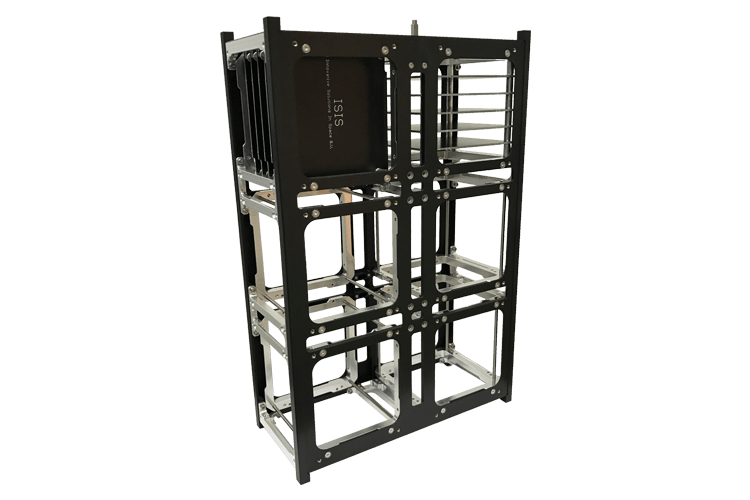
\includegraphics[scale=0.3]{gfx/structure.png}
    \caption{6U CubeSat Structure}
\end{figure}

\section{Sensors Parameters}
The spacecraft is equipped with three single axis gyroscopes and a three axis magnetometers which will be used to perform the full attitude determination.\\
The chosen sensor are the NSS Magnetometer available at cubesatshop.com and the Sensonor STIM 210 Gyroscope in the single axis configuration.\\
In table \ref{tab:magnetometers} and \ref{tab:gyroscopes} are reported the characteristics of the sensors chosen for the S/C.\\

\subsubsection{Magnetometer}
\begin{table}[H]
	\centering
	\begin{tabular}{|c|c|}
        \hline
        Orthogonality & +/- \ang{1} \\
        \hline
        Measurement Range & \SIrange{-60.000}{+60.000}{\nano\tesla} \\
        \hline
        Update rate & < \SI{18}{hz} \\
        \hline
        Resolution & < \SI{8}{\nano\tesla} \\
        \hline
         Noise density & < \SI{16}{\nano\tesla} \ {rms/hz} @ 1 Hz \\ 
        \hline
        Dimensions & \SI{96}{\milli\meter}x\SI{43}{\milli\meter}x\SI{17}{\milli\meter} \\
        \hline
        Mass & < \SI{85}{\gram} \\
        \hline
        Power & < \SI{750}{\milli\watt} \\
        \hline
        Thermal (operational) & \SIrange{248.15}{343.15}{\kelvin} \\
        \hline
        Radiation & \SI{10}{krad} \\
        \hline
        Power supply & +5V DC \\
        \hline
        Data & RS-485 \\
        \hline
        Connector & 9-pin Female Micro-D \\
        \hline
	\end{tabular}
	\caption{NSS Magnetometer by spacecraftshop}
	\label{tab:magnetometers}
\end{table}

\smallskip

\begin{figure}[H]
 	\centering
 	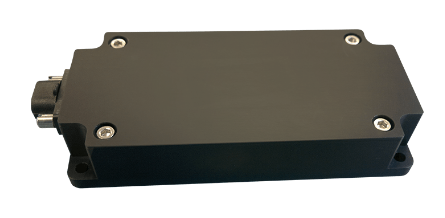
\includegraphics[scale=0.6]{gfx/NSSmagnetometer.png}
    \caption{NSS Magnetometer}
\end{figure}

\subsubsection{Gyroscope}
\begin{table}[H]
	\centering
	\begin{tabular}{|c|c|}
        \hline
        Measurement Range & +/- \ang{400}/s \\
        \hline
        Update rate & \SI{1}{hz} \\
        \hline
        Output & \SI{24}{bit} \\
        \hline
        Bias instability & \ang{0.3}/h \\ 
        \hline
        Angular radom walk & \ang{0.15}/$\sqrt{h}$ \\         
        \hline
        Dimensions & \SI{44.8}{\milli\meter}x\SI{38.6}{\milli\meter}x\SI{21.5}{\milli\meter} \\
        \hline
        Mass & < \SI{52}{\gram} \\
        \hline
        Power & < \SI{1500}{\milli\watt} \\
        \hline
        Thermal (operational) & \SIrange{218.15}{363.15}{\kelvin} \\
        \hline
        Radiation & \SI{10}{krad} \\
        \hline 
        Power supply & +5V DC \\
        \hline
        Data & RS-422 \\
        \hline
        Connector & 9-pin Female Micro-D \\
        \hline
	\end{tabular}
	\caption{Sensonor STIM 210 Gyroscope}
	\label{tab:gyroscopes}
\end{table}

\begin{figure}[H]
 	\centering
 	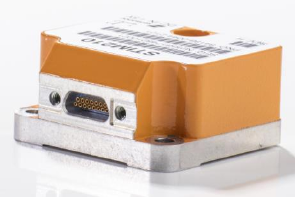
\includegraphics[scale=0.6]{gfx/STIM210.png}
    \caption{Sensonor STIM 210 Gyroscope}
\end{figure}

\section{Actuators Parameters}
The spacecraft is equipped with three magnetic torquers and a reaction wheel. Both the three magnetic torquers will be used to control the attitude of the spacecraft during the initial detumbling phase. The reaction wheel coupled with two magnetic torquers will be used to control the spacecraft during the Earth pointing phase. \\
The chosen actuators are the NCTR-M012 Magnetorquer Rod and the MAI-400 Reaction Wheel available at cubesatshop.com.\\
In table \ref{tab:magnetictorquer} and \ref{tab:reactionwheel} are reported the characteristics of the sensors chosen for the S/C.\\

\subsubsection{Magnetic Torquer}
\begin{table}[H]
	\centering
	\begin{tabular}{|c|c|}
        \hline
        Magnetic Moment & \SI{1.2}{\ampere\meter^2}\\
        \hline
        Linearity & +/- 5\% \\
        \hline
        Residual moment & < \SI{0.002}{\ampere\meter^2}\\
        \hline
        Operating range & \SIrange{263.15}{323.15}{\kelvin}\\
        \hline
        Power & \SI{800}{\milli\watt}\\
        \hline
        Random vibration & 14gRMS \\
        \hline
        Weight & \SI{50}{\gram}\\
        \hline
        Dimensions & \SI{94}{\milli\meter}x\SI{15}{\milli\meter}x\SI{13}{\milli\meter} \\
        \hline
        Power supply & +5V DC \\
        \hline        
	\end{tabular}
	\caption{NSS NCTR-M012 Magnetorquer Rod by spacecraftshop}
	\label{tab:magnetictorquer}
\end{table}

\smallskip

\begin{figure}[H]
 	\centering
 	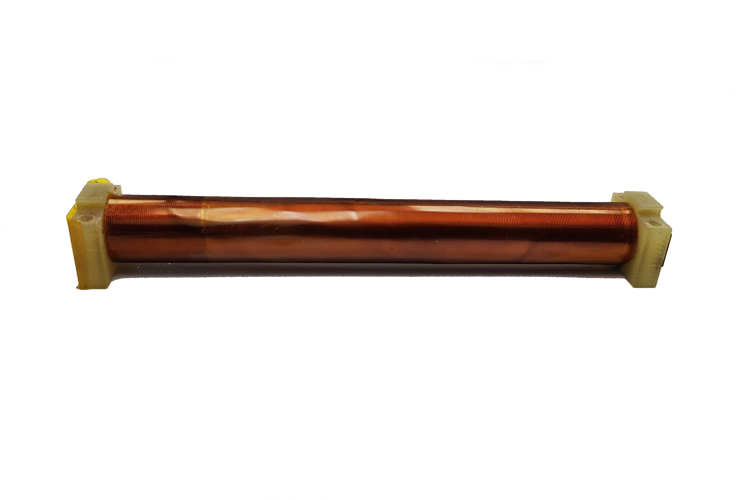
\includegraphics[scale=0.25]{gfx/magnetorquer.png}
    \caption{NSS NCTR-M012 Magnetorquer Rod}
\end{figure}

\subsubsection{Reaction Wheel}
\begin{table}[H]
	\centering
	\begin{tabular}{|c|c|}
        \hline
        Momentum Storage & \SI{11.076}{\meter\newton\meter\second} @ 10.000 RPM \\
        \hline
        Maximum Torque & \SI{0.635}{\meter\newton\meter} \\
        \hline
        Rotor Balance & < \SI{40}{\milli\gram\milli\meter} \\
        \hline
        Peak Current & \SI{440}{\milli\ampere} \\ 
        \hline
        Steady State Current & \SI{170}{\milli\ampere}  \\         
        \hline
        Idle Current & \SI{90}{\milli\ampere}  \\         
        \hline        
        Dimensions & \SI{330}{\milli\meter}x\SI{330}{\milli\meter}x\SI{384}{\milli\meter} \\
        \hline
        Mass &  \SI{110}{\gram} \\
        \hline
        Power & < \SI{1500}{\milli\watt} \\
        \hline
        Thermal (operational) & \SIrange{233.15}{358.15}{\kelvin} \\
        \hline
        Power supply & +5V DC \\
        \hline
	\end{tabular}
	\caption{Maryland Aerospace MAI-400 Reaction Wheel}
	\label{tab:gyroscopes}
\end{table}

\begin{figure}[H]
 	\centering
 	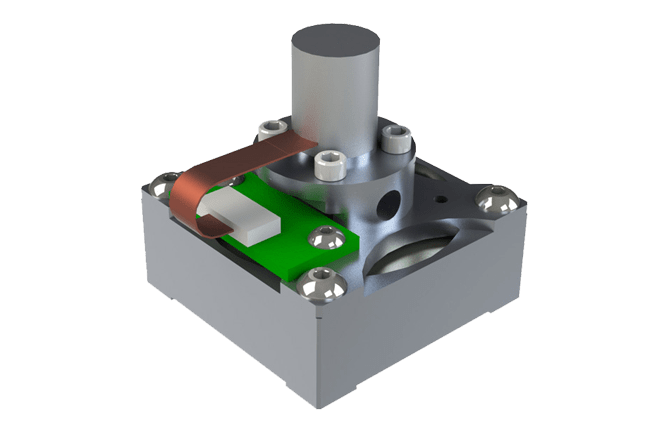
\includegraphics[scale=0.25]{gfx/mai_reaction_wheel.png}
    \caption{Maryland Aerospace MAI-400 Reaction Wheel}
\end{figure}

\section{External Disturbances Parameters}
To be able to correctly simulate the behavior of the external disturbances acting on the spacecraft the following parameters have been used : 

\begin{table}[H]
	\centering
	\begin{tabular}{|c|c|c|}
		\hline
		Parameters & Symbols & Values \\
		\hline	
		Planetary Gravitational Constant  & $\mu$ &  \SI{398600}{\kilo\meter^3/\second^2}\\
		\hline			
		Earth Radius & $R_e$ & \SI{6.378e+03}{\kilo\meter}\\
		\hline
		Earth Angular Velocity & $\omega_{e}$ & \SI{0.00007291}{\radian\per\second} \\
		\hline
	\end{tabular}
\end{table}

The departure date to correctly simulate the behavior of the external disturbances has been set to January 1st 2019, 12:00 AM.

\section{Spacecraft Parameters}
In this section are listed the parameters used to simulate the behaviour of the spacecraft.

\begin{table}[H]
	\centering
	\begin{tabular}{|c|c|c|}
		\hline
		Parameters & Symbols & Values \\
		\hline
		Total Mass & $M$ & \SI{12}{\kilo\gram}\\
        \hline
		First Principal Inertia Moment & $I_1$ & \SI{0.0612}{\kilo\gram\meter^2}\\
		\hline		
		Second Principal Inertia Moment & $I_2$ & \SI{0.1259}{\kilo\gram\meter^2}\\
		\hline
		Third Principal Inertia Moment & $I_3$ & \SI{0.1672}{\kilo\gram\meter^2}\\
		\hline
		Onboard Current Flow & $I$ & \SI{0.1}{\ampere}\\
		\hline
		Drag Coefficient & $C_d$ & 2.2 \\
		\hline
		Specular Reflection Coefficient & $\rho_{s}$ & 0.5 \\
		\hline
		Diffuse Reflection Coefficient & $\rho_{d}$ & 0.1 \\
		\hline
	\end{tabular}
\end{table}

The implicit assumption of perfectly adjustement and balance between the internal component has been made, in order obtain a rebalancing of the position of the center of mass corresponding to the center of main axis, so $CM_{X} = 0$, $CM_{Y} = 0$, $CM_{Z} = 0$.\\
A diagonal inertia tensor has been considered.\\

\chapter{Spacecraft Description}

\section{General Description}
In order to fullfill the mission required by the customer a CubeSat has been designed. \\
A CubeSat (U-class spacecraft) is a type of miniaturized satellite for space research that is made up of multiples of 10x10x10 cm cubic units. The CubeSat selected for the mission is made of 6 of those cubic units. \\
The CubeSat is equipped with a three axis magnetometer and three gyros as sensors which will be used to perform the attitude determination, and with four magnetic torquers and a reaction wheel to perform the attitude control.\\
The mission required from the customer is to perform Earth pointing.\\
The external surface of the CubeSat will be covered with solar panels in order to allow the spacecraft to generate enough power to be autonomous for the entire life of the mission : 

\begin{figure}[H]
 	\centering
 	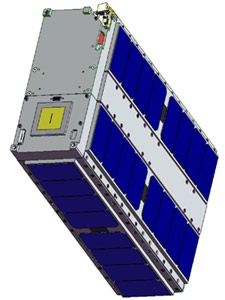
\includegraphics[scale=0.4]{gfx/cubesat_panels.jpg}
    \caption{6U CubeSat}
\end{figure}

\section{Sensors Description}
As stated before, the spacecraft is equipped with a three axis magnetometer and three gyroscopes to be able to determine and control the spacecraft attitude.
\subsection{Magnetometers}
Magnetometers have no moving parts and do not require a clear field of view.\\
They measure the sum of the ambient field that is of interest and
any local fields produced by the spacecraft. Local fields can be produced by
ferromagnetic materials or by current loops in solar arrays, electric motors, payload instruments, or most especially attitude control torquers. If the local fields are known, they can be compensated for. If they are not known, the magnetometers can be located far from the sources of magnetic contamination, on a deployable boom if necessary, to take advantage of the $1/r^3$ falloff of a magnetic dipole field. \\
They do require a well-modeled magnetic field if they are to be used as attitude sensors.\\
Nowadays for spacecraft applications MEMS Magnetometers are available.\\

\begin{figure}[H]
 	\centering
 	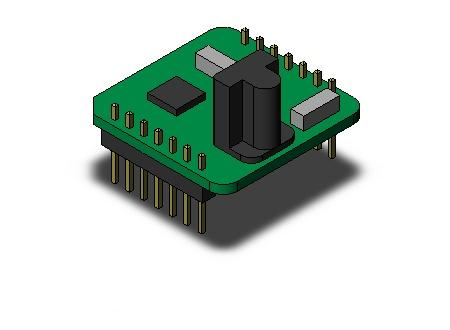
\includegraphics[scale=1]{gfx/magnetometer.jpg}
    \caption{MEMS Magnetometer}
\end{figure}

\subsection{Gyroscopes}
A gyroscope is any instrument which uses a rapidly spinning mass to sense and respond to changes in the inertial orientation of its spin axis.\\
In particular, rate gyros measure spacecraft angular rates and are frequently part of a feedback system for either spin rate control or attitude stabilization. The angular rate outputs from RGs may also be integrated by an onboard computer to provide an estimate of spacecraft attitude displacement from some initial reference. \\
All gyros have the basic construction geometry shown in Fig. \ref{fig:gyro}.\\
The angular momentum vector of a rate gyro is fixed in magnitude and parallel
to the gyro's spin axis. Because this vector maintains its inertial orientation in the absence of applied torques, spacecraft motion about the gyro's input axis causes the gimbal supporting the spin axis to precess about the output axis, or gimbal rotation axis. The output of an rate gyro is obtained from the motion of the gimbal.\\

\begin{figure}[H]
 	\centering
 	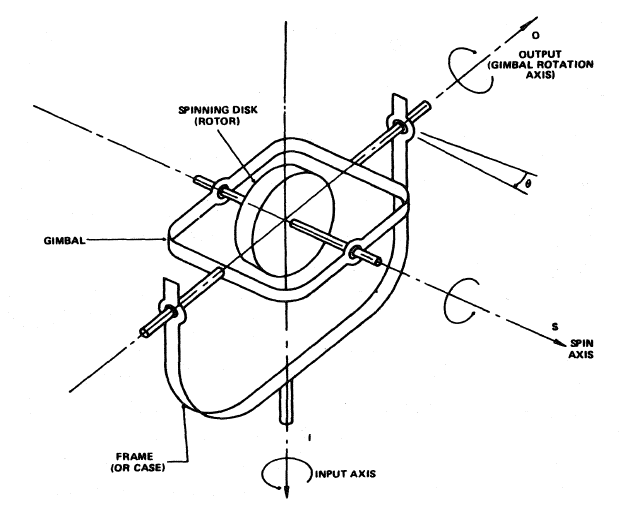
\includegraphics[scale=0.4]{gfx/gyroscope.png}
    \caption{Gyroscope}
    \label{fig:gyro}
\end{figure}

Rate gyros are the simplest and the least expensive gyros. Their accuracy is
generally suitable for spin rate control in a feedback system, but their integrated output requires frequent correction for precise attitude determination using other sensors such as Sun sensors or star trackers.\\
Errors in RG output are generally caused by nonlinearity, drift, and hysteresis. In addition, input accelerations may affect their accuracy if the gimbal is not perfectly balanced.\\
Nowadays for spacecraft applications MEMS gyros are available.\\

\begin{figure}[H]
 	\centering
 	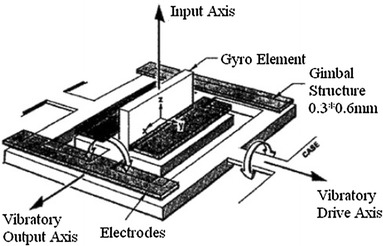
\includegraphics[scale=0.3]{gfx/mems_gyro.jpg}
    \caption{MEMS Gyroscope}
\end{figure}

\section{Actuators Description}
As stated in the general description, the spacecraft is equipped with three magnetic torquers and a reaction wheel in order to have full attitude control.
\subsection{Magnetic Torquers}
Magnetic torquers create a magnetic dipole moment, which in turn creates a
torque.\\
Magnetic torques can be used either directly for attitude control or to unload momentum accumulated by reaction wheels or control moment gyros. The simplest torquers are made of N turns of wire in a loop of area A; sending a current
I through such a coil produces a magnetic dipole moment in a direction perpendicular to the plane of the coil. \\
Most applications of magnetic torquers use three torquers producing moments
on orthogonal axes. It is generally not necessary to employ extra torque rods
for redundancy, because they usually have dual windings to provide internal
redundancy. 

\subsection{Reaction Wheels}
Reaction wheels are used as the primary attitude control actuators on most spacecraft for several purposes: 

\begin{itemize}
 \item add stability against disturbance torque;
 \item provide a variable momentum to allow operation for Earth-oriented missions;
 \item absorb cyclic torques;
 \item transfer momentum to the satellite body for the execution of slewing maneuvers;
\end{itemize}

These devices depend on the momentum of a spinning wheel.
Momentum-bias spacecraft may use one or two reaction wheels, but
full three-axis attitude control requires three or more wheels.\\

\section{Onboard Computer}
The onboard computer is the central core of the ADC system, and is responsible of acquiring data from sensors, performing attitude determination and control computation and drive the actuator by sending them the correct control variables.\\
The on board computer shall be able to exchange data with the ground station, collect informations about the health status of the spacecraft's sensors and actuators and perform housekeeping tasks.\\

\begin{figure}[H]
 	\centering
 	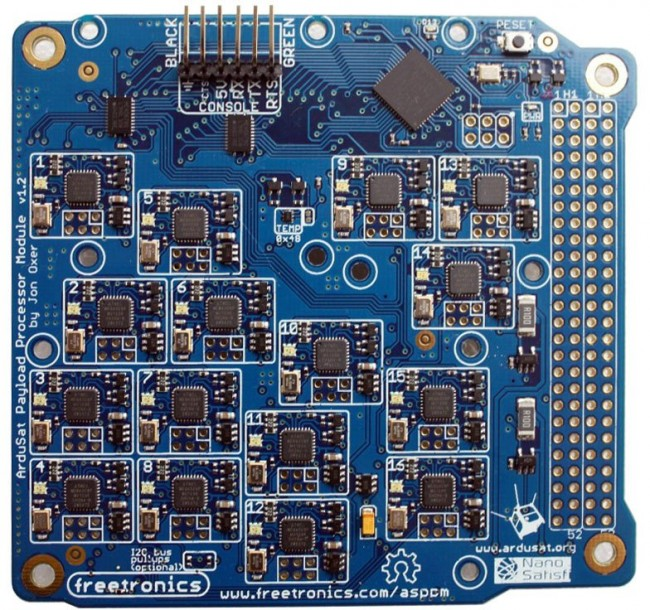
\includegraphics[scale=0.25]{gfx/ardusat.jpg}
    \caption{Ardusat On Board Computer}
\end{figure}

\section{Instruments and Actuators Placing}
The magnetic torquers are placed on the three principal axis of the spacecraft, while the reaction wheel is placed on the z-axis. The magnetometer is placed inside the spacecraft, while the three gyros are placed on the three principal axis of the spacecraft.

\begin{figure}[H]
 	\centering
 	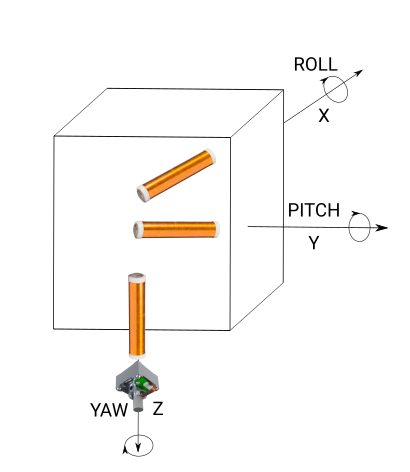
\includegraphics[scale=0.4]{gfx/actuators.png}
    \caption{Sensors and Actuators Placing}
\end{figure}

\section{ADCS Architecture}
The conceptual scheme of the ADCS architecture can be seen from Fig. \ref{fig:architecture}.\\
The four onboard sensors provide attitude measurement which are then processed on board in order to determine the attitude which then is passed to the controller.\\
The controller is responsible of sending the correct input to the actuators in order to obtain the desired attitude.

\begin{figure}[H]
 	\centering
 	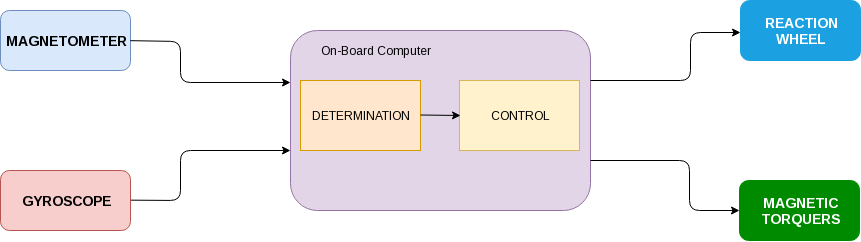
\includegraphics[scale=0.5]{gfx/adcs.png}
    \caption{ADCS Architecture}
    \label{fig:architecture}
\end{figure}

\section{Mass,Power and volume budget}

\subsubsection{Mass budget}

\begin{table}[H]
	\centering
	\begin{tabular}{|c|c|}
		\hline
		Components & Value \\
		\hline
		Structure & \SI{11}{\kilo\gram} \\
		\hline
	  	Sensors & \SI{0.241}{\kilo\gram}\\
		\hline
		Actuators & \SI{0.260}{\kilo\gram}\\
		\hline
		On-board Computer & \SI{0.035}{\kilo\gram}\\
		\hline
		Harness &  \SI{1}{\kilo\gram}\\
		\hline
        Others &  \SI{2}{\kilo\gram}\\
		\hline
		\textbf{Total} & \SI{14.536}{\kilo\gram}\\
		\hline 
	\end{tabular}
	\caption{Mass Budget}
\end{table}

\subsection{Volume budget}

\begin{table}[H]
	\centering
	\begin{tabular}{|c|c|}
		\hline
		Components & Value \\
		\hline
		Structure & \SI{110}{\milli\meter}x\SI{226}{\milli\meter}x\SI{340.5}{\milli\meter} \\
		\hline
	  	Magnetometer & \SI{96}{\milli\meter}x\SI{43}{\milli\meter}x\SI{17}{\milli\meter} \\
		\hline
	  	Gyroscope (x3) & \SI{96}{\milli\meter}x\SI{43}{\milli\meter}x\SI{17}{\milli\meter} \\
		\hline		
		Magnetic Torquers (x3) & \SI{94}{\milli\meter}x\SI{15}{\milli\meter}x\SI{13}{\milli\meter}\\
		\hline
		Reaction Wheel & \SI{330}{\milli\meter}x\SI{330}{\milli\meter}x\SI{384}{\milli\meter} \\
		\hline		
		On-board Computer & \SI{10}{\milli\meter}x\SI{5}{\milli\meter}x\SI{1}{\milli\meter}\\
		\hline 
	\end{tabular}
	\caption{Volume Budget}
\end{table}

\subsection{Power budget}

\begin{table}[H]
	\centering
	\begin{tabular}{|c|c|}
		\hline
		Components & Value \\
		\hline
	  	Magnetometer & \SI{0.7}{\watt} \\
		\hline
	  	Gyroscope (x3) & \SI{1.5}{\watt} \\
		\hline		
		Magnetic Torquers (x3) & \SI{0.8}{\watt} \\
		\hline
		Reaction Wheel & \SI{1.5}{\watt} \\
		\hline		
		On-board Computer & \SI{0.5}{\watt} \\
		\hline 
		\textbf{Total} & \SI{9.6}{\watt} \\
		\hline 		
	\end{tabular}
	\caption{Power Budget}
\end{table}

\chapter{Mathematical Modeling}

\section{Dynamics}
\subsection{Euler Equations}
The dynamics of a rigid body which is tumbling into space can be modeled by mean of the well known Euler equations : 

\begin{equation}
  \mathbf{\omega_B} = \mathbf{(I_B)}^{-1} [\mathbf{L_B} - \mathbf{\omega_b}  \wedge (\mathbf{I_B} \mathbf{\omega_b})
\end{equation}

where \textbf{$\omega_B$} is the angular velocity vector of the spacecraft in body frame, \textbf{$I_B$} is the inertia tensor of the spacecraft in body frame and \textbf{$L_B$} are the external torques acting on the spacecraft due to the external disturbances and the control action.\\

\subsection{Enviromental Disturbances}
The external disturbances acting on a LEO orbit spacecraft are basically four and are due to :

\begin{itemize}
  \item[-] Gravity Gradient
  \item[-] Magnetic Field 
  \item[-] Solar Radiation Pressure
  \item[-] Aerodynamic Drag
\end{itemize}

Details about how those torques have been mathematically modeled will be given in the following sections.

\subsubsection{Gravity Gradient}
Any nonsymmetrical rigid body in a gravity field is subject to a gravity-gradient torque.\\
It is usually adequate to approximate the gravity field as spherically symmetric for computing gravity-gradient torques. In this case, we have : 

\begin{equation}
 \mathbf{g(r)} = - \frac{\mu\mathbf{r}}{r^3}
\end{equation}

The gravity gradient torque about the center of mass therefore can be modeled as :

\begin{equation}
 \mathbf{L_{gg}} = \frac{3*mu}{r^3} \mathbf{n} \wedge (\mathbf{I} \mathbf{n})
\end{equation}

\subsubsection{Earth's Magnetic Field}
\subsubsection{Solar Radiation Pressure}
\subsubsection{Aerodynamic Drag}
\section{Kinematics}
\subsection{Euler Angles}
\subsection{Quaternions}
\section{Sensors Models}
\subsection{Magnetometer}
\subsection{Gyroscope}
\section{Actuators Models}
\subsection{Magnetic Torquers}
\subsection{Reaction Wheels}

\chapter{Determination}

\chapter{Control}
\section{B-Dot Control}
\section{Quaternion Feedback Control}
\section{Mixer Matrix}

\chapter{Simulink Model}

\chapter{Results}

\chapter{Conclusions}

\newpage
\end{document}
